\documentclass{article}
\usepackage[utf8]{inputenc}
\usepackage{graphicx}
\usepackage{subcaption}
\usepackage{geometry}
\geometry{left=38mm,top=30mm,bottom=30mm,right=25mm}
\usepackage{setspace}
\doublespacing
\begin{document}
\begin{titlepage}
\newcommand{\HRule}{\rule{\linewidth}{0.5mm}}

\center
\textsc{\LARGE \textbf{CMSC 6950 Open Science Project}}\\[1 cm]

\textsc{\Large Newfoundland and Labrador Aviation Wind Data}\\[0.5 cm]

\textsc{\large Jacob Newman (201528601)}\\[0.5 cm]





\vfill\vfill\vfill
{\large\today}
\vfill

\end{titlepage}

\begin{center}
\bf{Abstract}

Understanding historical climate data has become a major area of study across many fields in the past two decades. Graphical tools to depict climate data help scientists convey their information to the 
general public which in turn allows often complicate warnings to be easily understood by people not familiar with the topics. Here we discuss one of these tools, namely the Windrose Python package and 
apply it to wind data collected at airports around the province of Newfoundland and Labrador. We also show a way of connecting these polar diagrams to a mapping package (Basemap), which in turn provides 
a powerful way of connecting environmental factors to wind data interpretations.  

\end{center}
\section{Introduction}\label{Introduction}
Great strives to better understand and display historical climatological data have been made in the past two decades due to growing concerns over climate change among other things. One climatological 
data set that has a diverse range of importance when addressing these problems is wind data. Changes in major wind patterns, such as increases in the power of wind systems over time, can be used as a gauge to 
measure how the strength of storms is changing due to climate change \cite{Mendelsohn2012}. Another application of the study of wind data, in particular directional wind data, is designing wind power 
farms \cite{CETINAY201751} for a source of clean, renewable energy. For optimal placement of wind turbines, prominent wind directions and the associated wind speeds need to be plotted and 
analyzed. Other applications of studying wind data include mapping air pollution sources \cite{ADAMS2016133} and knowledge of dominant wind directions at airports, important information for 
pilots and air traffic controllers \cite{jairm26}.
\\
\indent Here we will look at the last of the applications in connection to airports in Newfoundland and Labrador. Wind speed and directional data are collected at each airport throughout the province, 
making data access relatively simple. A Python-based wind data visualization package Windrose \cite{Roubeyrie2018} will be employed to show several variations of polar diagrams used to plot each 
airport's respective wind data. Although we propose the purpose of this study to be that of knowledge gathering for pilots and air traffic controllers, a broad connection to the potential for wind 
energy production in the province of Newfoundland and Labrador (a long-discussed topic) can be made. We are merely limited by the availability of data to fully engage in the study of wind power 
potential. 
\\
\indent The remainder of this report is structured as follows, in section (\ref{Data_access}) we discusss data access and collection, in section (\ref{Wind_data_visualization}) we introduce the Windrose  
package and show multiple visualizations of directional wind data for a user-defined airport (see README), finally, in section (\ref{Discussion_and_conclusions}) we briefly discuss and conclude on some 
key points.      

\section{Methodology}\label{Methodology}

\subsection{Data Access}\label{Data_access}
The README file should be consulted for preliminary data access information and for instructions on how to call data from a particular airport. Here we talk about where the data is from and how it is 
collected. All the data (fifteen sets) available from the windData repository was accessed through the Canadian Climate Data Accessibility Portal (CCDAP). The CCDAP is a public data query platform that 
holds Canadian historical climate data collected and maintained by Environment and Climate Change Canada. CCDAP was made at the Water Security and Climate Change Lab (WSCC) at Concordia University. As 
mentioned above, each data set was collected at an airport in Newfoundland and Labrador over some range of time (given in the data set name). The data has been stripped to only include data/time, wind 
speed and wind direction information; full data sets for each locality include multiple additional weather measures such as temperature and visibility. The decision to only include wind data in this 
report (as other data, visibility, in particular, is also important information for air travel) was for two main reasons, firstly, the CCDAP limits the size of data sets and thus including additional 
weather measurements would restrict the range of time of each data set subsequently degraded the historical aspect of the information gathered by this study. Secondly, the Windrose package currently provides 
no mechanism for analyzing weather data other than wind data.
\\
\indent Each data set was collected by an aviation weather station. Since the age range of all the data is quite broad, no one system was used to collect each data set. We will therefore briefly 
discuss a commonly used aviation weather station, the Automated Weather Observation System (AWOS) shown in figure (\ref{AWOS}). AWOS is a core component of NAV Canada's weather monitoring system with 
over 100 systems in place across the country. Each system is installed on the airfield and collects weather data (e.g. wind speed and direction) continuously, in real-time and sends the information 
directly to the airport and pilots. This weather data is then stored and accessed via public portals such as CCDAP for a variety of studies such as this one. 

\begin{figure}[h!]
\centering
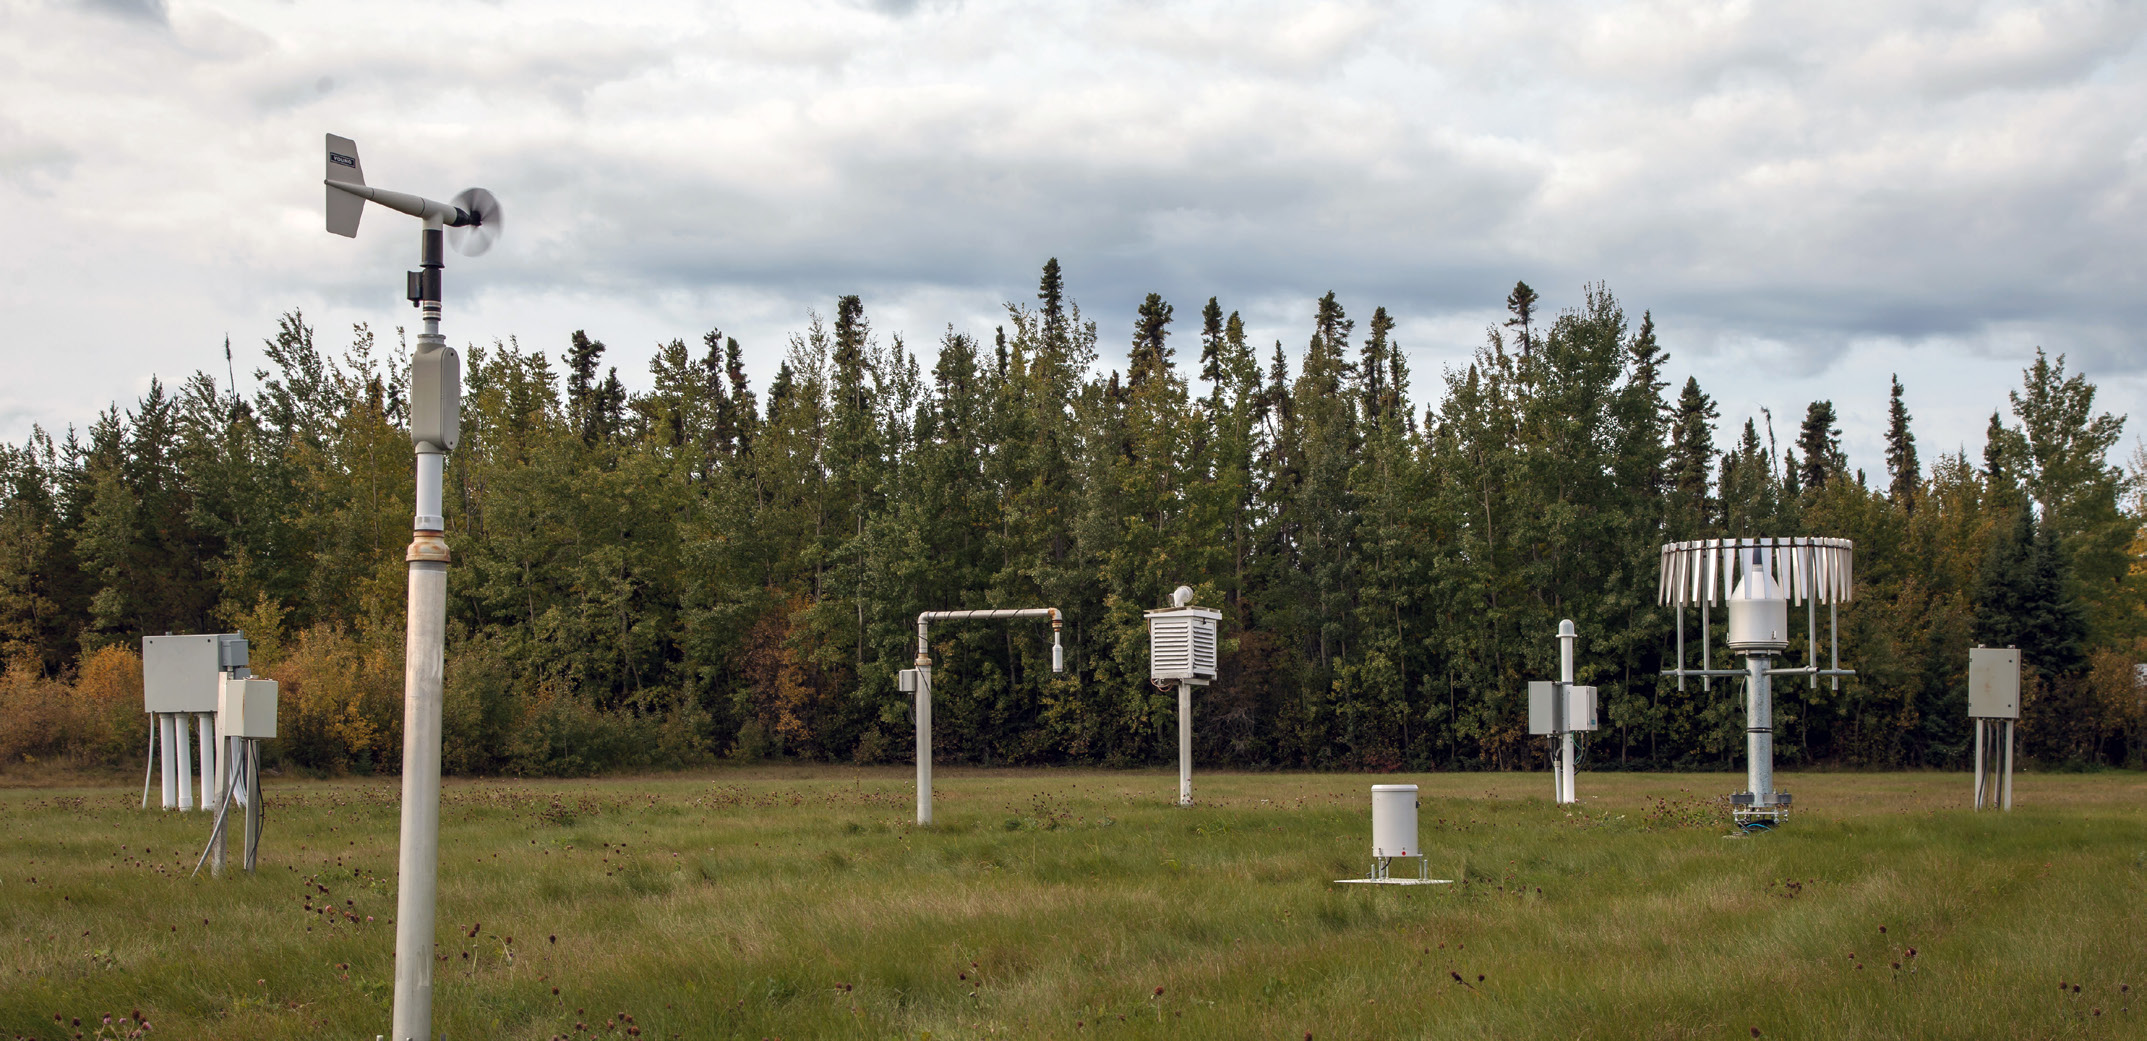
\includegraphics[width=10cm]{Images/AWOS.jpg}
\caption{Automated Weather Observation System (AWOS) used to monitor the weather at many airports throughout Canada. Older data sets or data sets from remote areas would have been collected on a 
similar, less-advanced weather station. Figure from NAV Canada.}
\label{AWOS}
\end{figure}

\subsection{Wind Data Visualization}\label{Wind_data_visualization}

The Windrose package is a graphic tool used to give a view of how wind speed and direction are typically distributed at a particular location (Roubeyrie and Cellers, 2018). The package is backended by 
Matplotlib to produce multiple polar (rose) diagrams for a given data set. These Windrose diagrams can subsequently be used in applications mentioned in section (\ref{Introduction}), among others. When 
these diagrams are tied with positional diagramats, such as the one seen in figure (\ref{location}) showing the location of the data presented in this report, links can be made between environmental 
aspect 
(wind tunnel effects, proximity to oceans, etc.) and the preferred wind directions.

\begin{figure}[h!]                                                                                                                                                                                                 
\centering                                                                                                                                                                                                         
\includegraphics[width=10 cm]{location.pdf}                                                                                                                                                                       
\caption{Map of Newfoundland and Labrador annotated by the location of wind data collection (yellow star). Other potential locations marked by black circles.}                                                                                                              
\label{location}                                                                                                                                                                                                   
\end{figure}

\indent Four main Windrose diagrams are offered with the package. The directional wind data for the user-defined location are plotted below with each variation of the Windrose diagrams. In figure 
(\ref{bar}), a bar polar diagram is shown, where the direction of the wind is depicted by the azimuthal direction of each bar. The outward extent of each bar represents the amount of wind direction 
measurements that resulted in each respective direction. Finally, the colour scheme of the bars represents the range of wind speeds observed in each direction. Figure (\ref{box}) is similar to figure 
(\ref{bar}) differing only in the frequency representation, being a box plot rather than a bar plot. Figures (\ref{contour}) and (\ref{contourf}) are the contour and filled contour Windrose diagrams 
respectively, representing direction, speed, and frequency by the azimuthal position, colour, and distance from the centre of the contours. The filled and un-filled contours can also be used together to 
better define the contours while still filling in the areas between them.
\\
\indent As the plots are dependent on the data set chosen by the user no attempt will be made to interpret and describe a particular Windrose diagram, similarily we will not describe each data set as 
there are fifteen potential locations which would result in quite a lengthy, repetitive process. The main take away from this section is the use of the Windrose diagrams to present the Newfoundland and 
Labrador aviation wind data and the potential application these plots have when used congruently with some type of location plot such as the map shown in figure (\ref{location}).
   
\begin{figure}[h!]
\centering
\includegraphics[width=9cm]{bar.pdf}
\caption{Directional wind data from a user-defined Newfoundland and Labrador airport plotted on a bar polar diagram from the Windrose Python package.}
\label{bar}
\end{figure}

\begin{figure}[h!]
\centering
\includegraphics[width=9cm]{box.pdf}
\caption{Directional wind data from a user-defined Newfoundland and Labrador airport plotted on a box polar diagram from the Windrose Python package.}
\label{box}
\end{figure}

\begin{figure}[h!]
\centering
\includegraphics[width=9cm]{contour.pdf}
\caption{Directional wind data from a user-defined Newfoundland and Labrador airport plotted on a contour polar diagram from the Windrose Python package.}
\label{contour}
\end{figure}

\begin{figure}[h!]
\centering
\includegraphics[width=9cm]{contourf.pdf}
\caption{Directional wind data from a user-defined Newfoundland and Labrador airport plotted on a filled contour polar diagram from the Windrose Python package.}
\label{contourf}
\end{figure}

\clearpage
\section{Discussion and Conclusions}\label{Discussion_and_conclusions}
The study of historical wind data for a particular location can provide insist in to several climate topics, among other things. Some of these topics include gauging the rate of climate change, air 
pollutant mapping, optimization of wind turbine placement, and information about airport wind patterns for air transportation safety. Here we provide a way to access wind data from the airports in 
Newfoundland and Labrador and applying this data to several polar diagrams from the Windrose Python package. These plots include bar, box, contour and filled contour polar diagrams that display how wind 
speed and direction are typically distributed at a particular airport. We also include a way of plotting the location of each airport on a map using the Basemap Python package. Using the Windrose 
diagrams, together with maps provides a powerful way of connecting wind patterns in a particular location to environmental influences. Using this workflow, with an increased data density from 
Newfoundland and Labrador opens a research avenue to answers the question of whether large-scale wind energy production could be feasible in the province.

\clearpage 
\bibliographystyle{unsrt}
\bibliography{main}
\end{document}
